% master.tex : master-fil for projektet
% ------------------------------------------------------------------------------
% Dette er hovedfilen for projektet, hvori indhold fra alle input-filer (tekst,
% billeder, litteraturdatabaser, osv.) samles

% Dokumenttypen 'book' er valgt pga. dens mange fleksible indstillinger
% Se https://tex.stackexchange.com/a/36989/118167
\documentclass[11pt,a4paper,twoside,openright,danish]{book}

% Variabler, som bruges til automatisk at indsætte titel, forfattere, osv. på
% forsiden og titelbladet.
\def \projecttitle       {Projekttitel}
\def \projectsubtitle    {Projektundertitel}
\def \projecttheme       {Projekttema}
\def \projectdegree      {Matematik}  % eller Matematik-Økonomi/Teknologi
\def \projectperiod      {Efterårssemesteret 20XX}
\def \projectnumber      {P1}
\def \projectgroup       {X123}
\def \projectauthors     {
  Sigrid\\
  Projektforfatter 2\\
  Projektforfatter 3\\
  Projektforfatter 4
  % ...
}
\def \projectsupervisors {
  Projektvejleder 1\\
  Projektvejleder 2
  % ...
}

% Preamblet indeholder alle de indstillinger og makroer, som skal indsættes for
% hovedindholdet, og i denne skabelon samles det i filen aaumath.sty, som
% definerer en pakke, der kan indlæses med \usepackage.
\usepackage{aaumath}

% Dokumentets indhold indsættes mellem \begin- og \end-makroerne for
% 'document'-blokken
\begin{document}

% Dokumentets 'front matter' tælles ikke med ifm. antal sider og nummereres med
% romerske tal. Herunder hører f.eks. forsiden, titelbladet, forordet og
% indholdsfortegnelsen.
\frontmatter
% incl/misc/frontpage.tex : rapportens forside
% ------------------------------------------------------------------------------


\backgroundsetup{
  scale = 1,
  angle=0,
  opacity=1,
  contents = {
    
\includegraphics[width=\paperwidth,height=\paperheight]{fig/img/aau/waves.pdf}
  }
}
\BgThispage
\pdfbookmark[0]{Forside}{forside}
\begin{titlepage}
  \centering
  \phantom{}
  \vspace{2cm}

  % AAU-segl
  \begin{minipage}[c]{0.2\paperwidth}
    \centering
    \makebox[0pt]{
      % fig/tikz/aau-badge.tex : AAU-logo til forsiden
% ------------------------------------------------------------------------------

\begin{tikzpicture}
  % Tegn hvid cirkel og tilføj det gennemsigtige, blå logo ovenpå
  \node[circle,color=white,fill=white,minimum size=1.175\textwidth] at (0,0) {};
  \node at (0,0) {
\includegraphics[width=\textwidth]{fig/img/aau/logo-circle.pdf}};
\end{tikzpicture}

    }
  \end{minipage}

  % Hovedindhold
  \vspace{4cm}
  {\fontfamily{bch}\selectfont
    \fboxsep0pt\colorbox{white}{
      \begin{minipage}{\textwidth}
        \centering
        \color{AAUblue1}

        \vspace{2em}
        {\Huge\bfseries\projecttitle}

        {\Large\bfseries\projectsubtitle}

        \bigskip
        \parbox{\textwidth}{\centering\large\projectauthors}

        \bigskip
        {\bfseries\large{\projectnumber}-Projekt, Gruppe \projectgroup, \projectdegree}
        \vspace{2em}
      \end{minipage}
    }
  }

\end{titlepage}

% incl/misc/titlepage.tex : rapportens titelblad
% ------------------------------------------------------------------------------
% Titelbladet genereres af makroen \aautitlepage, som er defineret i
% /incl/pre/ext/aautitlepage.sty


\pdfbookmark[0]{Titelblad}{titelblad}
\aautitlepage{
  \projectinfo{
    \projecttitle
  }{
    \projecttheme
  }{
    \projectperiod
  }{
    Gruppe \projectgroup
  }{
    \parbox[t]{\textwidth}{\projectauthors}
  }{
    \parbox[t]{\textwidth}{\projectsupervisors}
  }{
    \today
  }
}{
  \textbf{Institut for Matematiske Fag}\\
  Skjernvej 4A\\
  DK-9220 Aalborg Ø\\
  \href{http://math.aau.dk}{http://math.aau.dk}
}{
  % incl/misc/abstract.tex : projektets abstract
% ------------------------------------------------------------------------------
% Et abstract er et kort resume af rapporten, som vises på titelbladet

}

% incl/misc/contents.tex :
% ------------------------------------------------------------------------------

\pdfbookmark[0]{Indhold}{indhold}

% Indstillingerne i denne fil er grupperet, så de ikke påvirker andre dele
\begingroup

% Slå twoside fra midlertidigt for at undgår sideskift
\makeatletter
\@twosidefalse
\makeatother

% Placer indholdsfortegnelsen på sin egen side (bedst når den kun fylder en side)
\tableofcontents
\clearpage

% Placer oversigtslisterne på efterfølgende sider
\let\clearpage\relax
\listoffigures
\listoftables
\listofalgorithms
\lstlistoflistings

\endgroup


% Dokumentets 'main matter' (hovedindhold) er der, hvor det meste indhold skal
% sættes ind. Sider og overskrifter er nummererede med arabiske tal.
\mainmatter

% Input-filer bør opdeles således, at hver fil svarer til et kapitel. Makroen
% \include indsætter et sideskift og indholdet fra den givne stil.

% \include{incl/main/example1}
% \include{incl/main/example2}
% ...

\chapter{Indledning}
I dette mini-projekt, er problemet om en flyvemaskinekø i en lufthavn blevet introduceret.
Denne lufthavn har blot én landingsbane, hvilket kan skabe problemer hvis der er mange fly.
I dette projekt vil der blive konstrueret modeller for ankomsttiderne for fly, samt den tid det tager for fly at lande.
Der vil også blive simuleret en kø, for de fly der skal vente i luften for at lande.
Til slut vil resultaterne for simulationerne blive diskuteret, og på baggrund af disse resultater, vil der blive givet en anbefaling for hvorvidt lufthavnen skal tilføje en landingsbane mere, for at kunne følge med en 5\% årlig stigning af fly.

Når vi henviser til et program i dette projekt, kan det både findes i den tilhørende zip-fil, eller bagerst i rapporten som en del af appendix.

\section{Problemanalyse}
Som nævnt har den givne lufthavn blot én landingsbane, hvilket kan skabe kø. Opgivet er data for en "typsik" dag, hvilket inkluderer tiden mellem ankomster (i sekunder) og landingstider (i sekunder).
I Tabel \ref{tabel:intro_data} ses et udsnit af denne data.

\begin{table}[h]
	\centering
	\begin{tabular}{ c c c c c}
		\cline{1-2} \cline{4-5}
		Inter-arrival time [s]	&	Number of aircraft	&	\quad	&	Landing duration [s]	&	Number of aircraft	\\
		\cline{1-2} \cline{4-5}
		$0 - 59$								&	$44$								&				&	$0 - 30$							&	$0$									\\
		$60 - 119$							& $34$								&				&	$31 - 60$							&	$16$								\\
		$120 - 179$							& $27$								&				&	$61 - 90$							&	$33$								\\
		$180 - 239$							&	$22$								&				&	$91 - 120$						&	$61$								\\
		$240 - 299$							& $16$								&				&	$121 - 150$						&	$41$								\\
		$\vdots$								& $\vdots$						&				&	$\vdots$							&	$\vdots$						\\
		\cline{1-2} \cline{4-5}
	\end{tabular}
	\caption{Udsnit af det givne data for antallet af fly og tiden mellem deres ankomster og deres landingstid. Alt data kan ses i opgavebeskrivlesen.} \label{tabel:intro_data}
\end{table}

Dette data beskriver en "typisk" dag for lufthavnen. Hvis antallet af fly summeres, giver det i begge tilfælde 200 fly. Lufthavnen forventer en årlig stigning på 5\% af fly der lander på én dag. Det må betyde, at der på en typisk dag det første år lander 200 fly, mens der på en typisk dag i året efter lander 210 fly. Når denne stigning fortsætter vil flyene naturligt ankomme hurtigere efter hinanden, hvilket medfører en større kø og mere ventetid for flyene. Da skal det undersøges om denne ventetid kan reduceres ved at udvide lufthavnen med endnu en landingsbane, eventuelt efter nogle år, eller om lufthavnen fortsat kan klare presset mange år ude i fremtiden.

For at komme med en anbefaling til lufthavnsbestyrelsen skal denne data først analyseres. På baggrund af denne analyse skal der opstilles en model for at simulere flyankomster og landingstider på en given dag i et givent år.
Denne givne dag skal da afvikles i en kø-simulering ,både med én og to landingsbaner, og ventetiden vil da kunne simuleres.
Disse simuleringer skal køres for mange dage i et givent år, og igen for mange forskellige år for at udregne en gennemsnitelig ventetid for en dag i et år.

I dette projekt vil der blive brugt programmeringssproget Python, da det er et anerkendt og meget populært sporg. Desuden bliver det brugt af både programmøre, videnskabsmænd og matematikere. Python er et Open-Source programmeringssprog hvor der eksisterer mange forskellige pakker der kan hentes og benyttes gratis. Desuden er Pyhton letlæselig sammenlignet med mange andre programmeringssprog (KILDE) og i 2019 rangerede det som nummer et på \textsc{IEEE}'s rangliste over de bedste programmeringssprog i verden. (KILDE)

Da må problemformuleringen for programmet, der skal køre simuleringen, være:

\begin{center}
	\textit{Lav en model for det givne data og skriv et progam i Python der skal simulere mange dage i de forskellige år og som kan udregne den gennemsnittelige ventetid for de forskellige år.
	På baggrund af disse resulater, skal der gives en anbefaling til lufthavnsbestyrelsen, om hvorvidt de skal udvide lufthavnen med endnu en landingsbane.}
\end{center}

\chapter{Modellering}
I projektet er der opgivet data for en "typisk" dag i form af et skema over hyppigheden af ankomsttider mellem fly og hyppigheden af landingsvarigheden for fly. For at kunne lave en simulering af flyankomster i en dag i lufthavnen, er det nødvendigt at analysere denne data, og eventuelt finde en model til at generere tiderne, som stemmer overens med den "typiske" dag.
\section{Ankomsttider}
Givet er data for hvor mange fly der ankommer inden for et specifikt interval efter det forrige fly. På baggrund af dette kan der genereres ankomsttider for en specifik dag det første år, og tiden det tager for alle fly at ankomme kan da beregnes.

En måde at gøre det på er, at generere først $44$ tilfældige tal mellem $0 - 59$, så $34$ tilfældige tal mellem $60 - 119$, osv. Alle disse ankomstider mellem flyene kan da lægges sammen, og denne sum må da være den tid det tager for alle 200 fly at ankomme.
I filen \code{arrival\_times.py} kan man se et \textsc{Python}-program der gør netop dette, og som printer antallet af fly og tiden i alt i timer.
Køres dette et par gange vil resultatet være, at der alle gange er 200 fly, men at tiden i alt vil varriere mellem $12 - 13.5$ timer.

Da tiden i alt varrierer, vælges det at køre programmet mange gange for da at tage gennemsnittet af alle kørsler.
I filen \code{arrival\_times\_mean.py} findes et \textsc{Python}-program der udfører netop dette, og som printer gennemsnittet. Køres dette program $100,000$ gange (ved at sætte variablen \code{repetitions = 100000}) fås et gennemsnit på $12.9$ timer.

\subsection{Model for ankomsttider} \label{chap:model_arrival_times}
Det kunne forestilles, at fly i en lufthavn ankommer uafhængigt af hinanden i løbet af den tid lufthavnen tager imod ankomster.
Derfor kunne en passende model måske være at ankomsttiderne er tilfældigt spredt på en tidslinje på $13$ timer.
Denne hypotese kan undersøges.
I programmet \code{plot\_inter\_arrival\_time\_model.py} gerereres der $200$ tilfældige sekunder i tidsintervallet fra $0 - 13$ timer, der så sorteres. Dette må være en liste over ankomstiderne med denne model.
Da udregnes ankomsttiderne mellem flyene, og der tælles op, hvor mange ankomsttider mellem flyene der er i de givne intervaller.
Dette gentages mange gange, og der bliver taget en gennemsnit af alle antallene hvilket til sidst plottes.

I Figur \ref{fig:given_arrival_time_plot} ses de givne data for ankomsttider på en typisk dag plottet i et histogram, mens der i Figur \ref{fig:model_arrival_time_plot} ses gennemsnittet for de genererede ankomsttider med modellen plottet i et histogram.

\begin{figure}[h!]
	\centering
	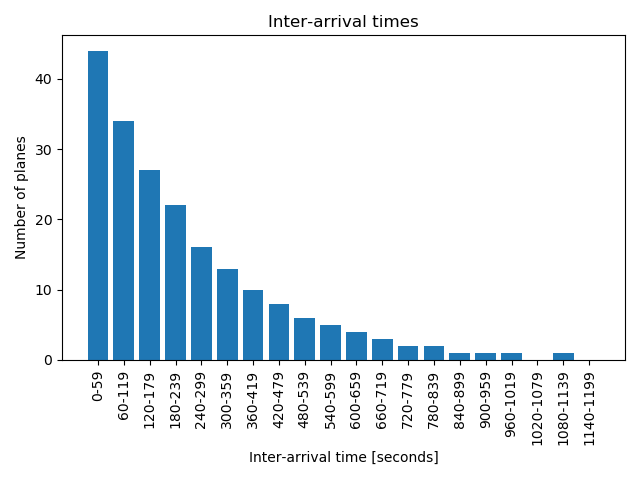
\includegraphics[scale=0.7]{fig/img/given_arrival_time_plot.png}
	\caption{Plot over det givne datasæt for ankomsttimer} \label{fig:given_arrival_time_plot}
\end{figure}

\begin{figure}[h!]
	\centering
	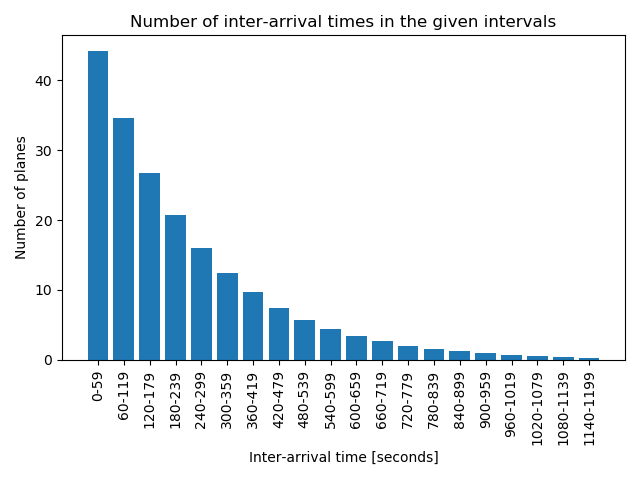
\includegraphics[scale=0.7]{fig/img/model_arrival_time_plot.png}
	\caption{Plot over gennemsnittet af antal for de generede ankomsttimer med modellen} \label{fig:model_arrival_time_plot}
\end{figure}

Det er tydeligt at modellen er god for ankomsttiderne. Da må ankomsttiderne for flyvemaskinerne i lufthavnen kunne simuleres, ved tilfældigt at plotte dem på en tidslinje fra $0 - 13$ timer.

\section{Landingsvarigheder}
Landingsvarighed er den tid (i sekunder) et fly bruger på at lande.
Altså er landingsbanen fri når landingsvarighed for et fly er gået.
Igen er det givne data for en "typisk" dag en tabel over tidsintervaller, og det antal fly hvis landingsvarighed ligger inden for det. Igen summerer antallet af fly til 200. I Figur \ref{fig:given_landing_durations_plot} ses et histogram over antallet af fly og landingsvarighederne.

\begin{figure}[h!]
	\centering
	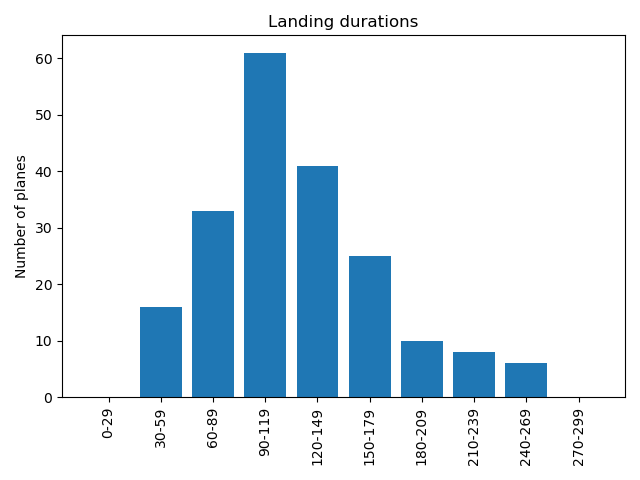
\includegraphics[scale=0.6]{fig/img/given_landing_durations_plot.png}
	\caption{Plot over det give data for landingsvarighederne.} \label{fig:given_landing_durations_plot}
\end{figure}

Det ses i Figur \ref{fig:given_landing_durations_plot} at fordelingen er forskellig fra ankomsttiderne.
Fordelingen ligner til dels en normalfordeling, da der på samme måde som i en normalfordeling er en "pukkel".
Dog er fordeligen for landingsvarighederne ikke symmetrisk omkring det højeste punkt, som en normalfordeling er, og ligner derfor mere en "skæv" normalfordeling.

Det har i projektet ikke været muligt at finde en model der passer på det givne data.
Desuden afviger landingsvarighederne sig fra ankomsttiderne, da landingsvarigheden direkte kan blive påvirket af udefrakommende paramentre.
Landingsvarigheden for et fly vil ikke bare være et tilfældigt tal inden for et tidsinterval, men vil kunne blive påvirket af eksempelvis den hastighed eller acceleration flyet lander med. 

Da der ikke er blevet fundet en model der passer til det givne data, må det blive nødvendigt at bruge netop de givne tidsintervaller til at generere tilfældige landingsvarigheder for en specifik dag. Den specifikke metode brugt i dette projekt beskrives i afsnit \ref{chap:landing_durations} i kapitel \ref{chap:program}.

\chapter{Køsimulering} \label{chap:queue}
Når flyene ankommer kan der opstå et tilfælde hvor et fly ankommer mens alle landingabaner er optagede.
I det tilfælde skal flyet der endnu ikke kan lande forblive i luften.
Dette er et eksempel på et køproblem. Den simpleste måde at løse problemet er altid at lade den forreste i køen lande, når en landingsbane bliver ledig.

Der er mange tilgange til at simulere en kø. I projektet blev der brugt (KILDE) som inspiration til en køsimulering med både én og flere landingsbaner.
I Figur \ref{fig:queue_flowchart} på næste side ses et flowchart som illustrerer den køsimulation der bliver brugt i dette projekt.

\begin{figure}
	\centering
	\scalebox{0.7}{
		\tikzstyle{startstop} = [rectangle, rounded corners, minimum width=3cm, minimum height=1cm,text centered, draw=black, fill=red!30]
\tikzstyle{io} = [trapezium, trapezium left angle=70, trapezium right angle=110, minimum width=3cm, minimum height=1cm, text centered, text width=4cm, draw=black, fill=blue!30]
\tikzstyle{process} = [rectangle, minimum width=4cm, minimum height=1cm, text centered, text width=4cm, draw=black, fill=orange!30]
\tikzstyle{decision} = [diamond, width=2cm, height=1cm, text centered, text width=2cm, draw=black, fill=green!30]
\tikzstyle{arrow} = [thick,->,>=stealth]

\begin{tikzpicture}[node distance=2cm]
	\node (start) [startstop] {Start};
	\node (pro1) [process, below of=start] {Sæt tiden og ventetiden lig nul, samt lad alle landingsbaner være tomme};
	\node (dec1) [decision, below of=pro1, yshift=-1cm] {Er alle fly landet?};
	\node (pro2) [process, below of=dec1, yshift=-1cm] {Beregn den næste ankomsttid};
	\node (dec2) [decision, below of=pro2, yshift=-1.5cm] {Er det næste event en ankomst?};
	\node (pro3a) [process, right of=dec2, xshift=3cm] {Sæt tiden lig den næste ankomsttid};
	\node (dec3a) [decision, right of=pro3a, xshift=3cm] {Er der en fri landingsbane?};
	\node (pro4aa) [process, right of=dec3a, xshift=3cm] {Land flyet her og udregn den næste tid en landing er færdig for denne bane};
	\node (pro4ab) [process, below of=dec3a, yshift=-1cm] {Placér flyet bagerst i køen};
	\node (dec4) [decision, below of=dec2, yshift=-5cm] {Er det næste event at en landingsbane bliver fri?};
	\node (pro5a) [process, right of=dec4, xshift=3cm] {Sæt tiden lig den næste tid til en landing er færdig};
	\node (dec5a) [decision, right of=pro5a, xshift=3cm] {Er der fly i køen?};
	\node (pro6aa) [process, right of=dec5a, xshift=3cm] {Tag det forreste fly ud af køen og land flyet her. Udregn den næste tid en landing er flrdig for denne bane, og opdater den samlede ventetid med ventetiden for dette fly};
	\node (pro6ab) [process, below of=dec5a, yshift=-1cm] {Sæt landingsbanen til at være tom};
	\node (out1) [io, below of=dec4, yshift=-4cm] {Udregn den gennemsnittelige ventetid og retuner denne};
	\node (stop) [startstop, below of=out1] {Stop};

	\node (dec4an) [above of=dec4, yshift=1cm];
	\node (dec1ana) [below of=dec4, yshift=-2cm, xshift=-4cm];
	\node (out1an) [above of=out1, xshift=18cm, yshift=-0.7cm];
	\node (nej1) [below of=dec4, anchor=east, yshift=-1cm] {Nej};
	\node (ja1) [right of=dec1, anchor=south] {Ja};
	
	\draw [arrow] (start) -- (pro1);
	\draw [arrow] (pro1) -- (dec1);
	\draw [arrow] (dec1) -- node[anchor=east] {Nej} (pro2);
	\draw [arrow] (pro2) -- (dec2);
	\draw [arrow] (dec2) -- node[anchor=south] {Ja} (pro3a);
	\draw [arrow] (pro3a) -- (dec3a);
	\draw [arrow] (dec3a) -- node[anchor=south] {Ja} (pro4aa);
	\draw [arrow] (dec3a) -- node[anchor=east] {Nej} (pro4ab);
	\draw [thick] (pro4aa) |- (dec4an);
	\draw [thick] (pro4ab) |- (dec4an);
	\draw [arrow] (dec2) -- node[anchor=east] {Nej} (dec4);
	\draw [arrow] (dec4) -- node[anchor=south] {Ja} (pro5a);
	\draw [arrow] (pro5a) -- (dec5a);
	\draw [arrow] (dec5a) -- node[anchor=south] {Ja} (pro6aa);
	\draw [arrow] (dec5a) -- node[anchor=east] {Nej} (pro6ab);
	\draw [thick] (pro6aa) |- (dec1ana);
	\draw [thick] (pro6ab) |- (dec1ana);
	\draw [arrow] (dec1ana) |- (dec1);
	\draw [thick] (dec4) |- (dec1ana);
	\draw [thick] (dec1) -| (out1an);
	\draw [arrow] (out1an) -| (out1);
	\draw [arrow] (out1) -- (stop);
\end{tikzpicture}

	}
	\caption{Flowchat der illustrer en køsimulering} \label{fig:queue_flowchart}
\end{figure}

I starten af simuleringen sættes en variabel hvor den samlede tid der er gået lig nul.
Desuden sættes også den samlede ventetid lig nul, og alle landingsbanerne sættes til at være tomme. Derefter startes en while-løkke, som først slutter når alle fly er landet.

I while-løkken tjekkes der for to centrale begivenheder (events).
Den ene begivenhed er at et nyt fly ankommer til lufthavnen, mens den anden begivenhed er at en landingsbane bliver ledig.
Hvis et nyt fly ankommer, skal det enten lande på en ledig landingsbane, eller også placeres bagerst i køen.
Hvis en landingsbane bliver ledig, skal det næste fly i køen lande, hvis ikke køen er tom, eller også skal landingsbanen opdateres som tom, hvis der ingen fly er i køen.
Hvis et fly har været i køen, skal den tid det har ventet i køen gemmes når det får lov til at lande. Denne ventetid bliver plusset til den samlede ventetid, og til sidst i simuleringen vil den gennemsnittelige ventetid per fly blive returneret. 
Hvis et et fly ikke har været i kø, har det ikke haft nogen ventetid, og da er det ikke nødvendigt at opdatere den samlede ventetid.

Denne simulation virker for ethvert antal af landingsbaner.
Derfor er det den samme der vil blive brugt både til tilfældet hvor der er én, og hvor der er to landingsbaner.

Køsimuleringen er en del af det større program der udregner den gennemsnittelige ventetid per fly på en dag hvert år.
Dette program kan findes som filen \code{airplanes.py}, og køsimuleringen er en funktion der heri starter på linje 45 kaldet \code{sim\_day()}.

\chapter{Programmet} \label{chap:program}
Det centrale program i dette projekt er en fil der er navngivet \code{airplanes.py}.
Dette program tager ingen input, og er delt op i en main-funktion, og otte andre underfunktioner.
Programmet udregner den gennemsnittelige ventetid per fly for en dag i alle år, og resultatet for hvert år bliver skrevet ud i en fil.

De fire centrale funktioner vil her blive gennemgået.

\section{Main-fuktionen}
I Kildekode \ref{code:main} ses et udsnit af programmet, der netop indeholder main-funktionen.

\begin{lstlisting}[language=Python, caption={Main-funktionen i airplanes.py}, label=code:main]
# Run the simulation and write the results to a file
if __name__ == "__main__":
    years = 15
    runways = 2
    avg_wait = simulate(runways, years, 300)
    write_results_to_file(avg_wait, years)
\end{lstlisting}

I starten af denne funktion defineres først de to vaiabler \code{years} og \code{runways}. Disse kan ændres alt efter hvor mange år simulationen skal simulere, og hvor mange landingsbaner lufthavnen har.
Derefter kaldes funktionen \code{simulate()}, hvis output bliver gemt i listen \code{avg\_wait}.
Denne liste består af den gennemsnittelige ventetid per fly for en dag i et år, og dens længde er da netop antallet af år, altså den værdi der er gemt i \code{years}.
Til slut kaldes funktionen \code{write\_results\_to\_file()}, der skriver disse resultater til en fil.

\section{Simulate-funktionen}
Udsnittet af denne funktion ses i Kildekode \ref{code:simulate} herunder.

\begin{lstlisting}[language=Python, caption={simulate-funktionen i airplanes.py}, label=code:simulate]
# Run the simulation and calculate number of planes each day in the year
def simulate(runways, years, sim_per_year):
    planes = 200
    avg_wait = []
    for i in range(years):
        avg_wait.append(sim_year(runways, round(planes), sim_per_year))
        planes *= 1.05
    return avg_wait
\end{lstlisting}

Funktionen tager tre input: Antallet af landingsbaner, antallet af år, og det antal simuleringer der skal køres for ét år.
Listen \code{avg\_wait} skal bestå af resultaterne for simuleringerne, og i hver gentagelse af for-løkken bliver funktionen \code{sim\_year} kaldt, hvis output skrives på en ny plads bagerst i listen.
Derefter stiger antallet af fly med de 5\%.
Til slut returneres \code{avg\_wait}.

\section{Simulering af dage i et år}
For at beregne et gennemsnit for ventetiden per fly på en dag for et år skal der køres mange simuleringer af en dag på det givne år.
Funktionen \code{sim\_year} i programmet kan ses i Kildekode \ref{code:sim_year}.
I løbet af denne funktion bliver funktionen \code{sim\_day} kaldt, og denne funktion består af den køsimulering der blev gennemgået i kapitel \ref{chap:queue}. 

\begin{lstlisting}[language=Python, caption={sim\_year-funktionen i airplanes.py}, label=code:sim_year]
# Run one day's simulationen sim_per_year times
def sim_year(runways, planes, sim_per_year):
    sum_of_avg_wait = 0    
    for sim in range(sim_per_year):
        schedule = generate_schedule(planes)
        sum_of_avg_wait += sim_day(runways, schedule)
    return sum_of_avg_wait/float(sim_per_year)
\end{lstlisting}

Funktionen \code{sim\_year} tager tre input, netop antallet af landingsbaner, antallet af fly dette år og antallet af simuleringer der skal køres for året.
I variablen \code{sum\_of\_avg\_wait} bliver summen af hver gennemsnittelig ventetid per fly for en dag gemt.
For-løkken gentages det antal gange køsimuleringen skal køres for et år, hvilket netop er det antal der er gemt i variablen \code{sim\_per\_year}.
For hver gentagelse skal der genereres en ny tidsplan, og en ny køsimulerign skal køres med denne tidsplan.
Til slut returneres gennemsnittet af den gennemsnittelige ventetid per fly for en dag.

En tidsplan er en liste af tubler, hvor der er én tubel for hvert fly der skal lande den dag, og hvor tublerne er ordnede efter ankomsten.
En tubel består af et flys ankomsttid (i sekunder), og flyets landingsvarighed (i sekunder).
Ankomsttid betyder her det præcise tidspunkt flyet ankommer, og er altså ikke en "inter-arrival time".
I tidsplanen er eksempelvis værdien \code{schedule[0][1]} lig landingsvarigheden for det første fly.

Funktionen \code{generate\_schedule} består blot af tre linjer.
Den første kalder funktionen \code{genera} \code{te\_arrival\_times}, som bruger modellen fra afsnit \ref{chap:model_arrival_times} til at generere en liste over alle ankomsttider.
Derefter bliver funktionen \code{generate\_landing\_durations} kaldt, der genererer en liste over landingsvarigheder, og til slut returneres de to lister "zippet" sammen.

\section{Generering af landingsvarigheder} \label{chap:landing_durations}
Siden hvert fly har en tid det tager for det at lande, skal der genereres en liste af landingsvarighed, hvor hver eneste flys landingsvarighed er gemt.

I det første år lander der 200 fly om dagen. Fra det givne data over en "typisk" dag fås det at der ud af de 200 fly er 16 fly der tager mellem $31 - 60$ sekunder at lande.
I det første år kan landingstiderne da genreres på det måde, at der bliver trukket 16 tilfældige tal mellem $31 - 60$ i første omgang, og derefter bliver trukket et antal nye tider inden for det interval antallet tilhører.
Til slut kan listen af alle disse tider blandes.

Når antallet af fly stiger bliver det dog lidt vanskligere.
Da kan der med fordel udregnes frekvensen af hyppigheden af fly hvis landingsvarighed falder inden for de forskellige intervaller.
Den kumulerede frekvens kan da udregnes for hvert af intervallerne.
Hvis der nu trækkes et tilfældigt tal mellem $0-1$ må det ligge mellem en af to kumulerede frekvenser, og da kan der trækkes en tilfældig landingsvarighed i det tidsinterval frekvensen svarer til.
Denne metode kan gentages for alle fly uanset antallet, og fordeligen af flyenes landingsvarighed vil da forblive den samme som det data der er blevet givet for en "typisk" dag. 

I Kildekode \ref{code:gen} ses løsningen som \textsc{Python}-kode.

\begin{lstlisting}[language=Python, caption={generate\_landing\_durations-funktionen i airplanes.py}, label=code:gen]
# Genreate a list of landing durations
def generate_landing_durations(planes):
    data = [0, 16, 33, 61, 41, 25, 10, 8, 6]
    min_ = 0
    max_ = 30
    model = [[0.0, 0, 30]]
    for index, num in enumerate(data[1:]):
        percent = float(num) / planes + model[index][0]
        min_ = 1 + max_
        max_ = 29 + min_
        model.append([percent, min_, max_])
    percent_list = [random.random() for i in range(planes)]
    landing_durations = []
    for percent in percent_list:
        for index in range(len(model) - 1):
            if model[index][0] < percent and percent <= model[index + 1][0]:
                landing_durations.append(random.randint(model[index + 1][1], model[index + 1][2]))
                break
    return landing_durations
\end{lstlisting}

I funktionen bliver det givne data for landingsvarigheden først gemt i listen \code{data}. Listen \code{model} består af lister, hvor det første element er den kumulerede frekvens, det næste er den mindste værdi i tidsintervallet, og den sidste den største værdi i tidsintervallet.
For hvert datapunkt i \code{data} (med undtagelse af det første) bliver der da udregnet en kumuleret frekvens og en min og max værdi for tidsintervallet, og disse gemmes i \code{model}. 
Derefter trækkes der det samme antal tilfældige tal mellem $0-1$ som der er fly, og disse gemmes i \code{percent\_list}.
For hver af disse værider bliver det tjekket hvilket tidsinterval de matcher, og der bliver da trukket et tilfældigt tal i dette interval, som bliver gemt i listen \code{landing\_durations}.
Til slut returneres denne liste.

\chapter{Resultat}
Fra programmet, gennemgået i kapitel \ref{chap:program}, fås der kun gennemsnittelige ventetider for hvert år skrevet i en tekstfil.
For at kunne sammenlige disse resultater når antallet af landingsbaner ændres, skal programmmet da køres flere gange hvor værdien \code{runways} ændres.

Programmet \code{plot.py} plotter et histogram med de filer som skrives som et command-line argument.
Med dette program er de to datasæt \code{15Y1K.txt} og \code{15Y2K.txt} (genereret med \code{airplanes.py}) blevet plottet, hvilket kan ses i Figur \ref{fig:results}.

\begin{figure}[h]
	\centering
	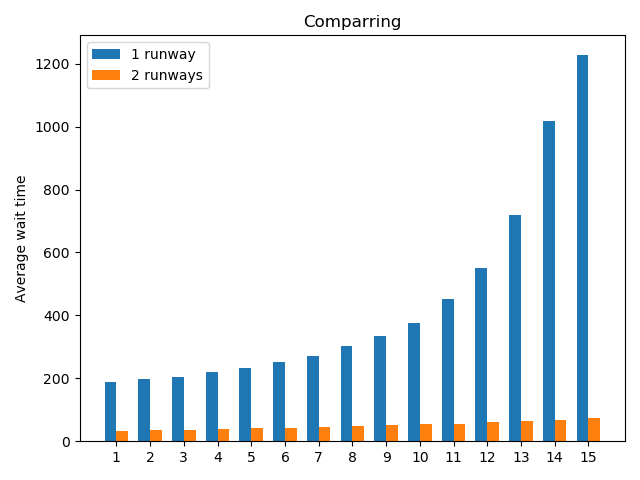
\includegraphics[scale=0.7]{fig/img/results_15Y.png}
	\caption{Et plot over den gennemsnittelige ventetid per fly over 15 år ved både én og to landingsbaner.} \label{fig:results}
\end{figure}

På figuren ses det tydeligt at to landingsbaner er en forbedring på den gennemsnittelige ventetid.
Ventetiden er på omkring 80 sekunder i det første år med én landingsbane, mens den for to er på omkring 6 sekunder.
Det kan også ses at ventetiden med én landingsbane efter mange år begynder at stige meget hurtigt, mens den med to landingsbaner bliver ved med at stige en lille smule i alle 15 år.
Generelt bliver ventetiden mere end ti gange så lille hvis der tilføjes en ekstra landingsbane.

En anbefaling til lufthavnsbestyrelsen må da være at det efter ti år vil blive nødvendigt at udvide landingsfaciliteterne, da flyene i gennemsnit vil komme til at vente omkring $6-7$ minutter med blot én landingsbane.
Dog vil det være en stor fordel for lufthavnen at udvide så hurtigt som muligt, da det altid vil forbedre ventetiden markant, hvilket vil resultere i mere tilfredse kunder.


% Appendicer indsættes inde i en appendices-blok og bliver nummereret med
% bogstaver i stedet for tal
\begin{appendices}
  % \include{incl/app/appendix1}
  % \include{incl/app/appendix2}
  % ..
\end{appendices}

% Dokumentets 'back matter' er til ekstra ting som f.eks. litteraturlisten.
% Overskrifter bliver ikke nummereret her.
\backmatter

% Automatisk litteraturliste baseret på, hvilke kilder, der er blevet refereret
% til i løbet af rapporten.
\bibliographystyle{apalike}
\bibliography{
  incl/bib/books,
  incl/bib/articles,
  incl/bib/software
}

\end{document}
